% =====================================================================
%  COMP 333 Project -- Phase 1 Report
%  Unified 2D Shape Classifier
%  Compile with:  pdflatex phase1_report.tex  (run twice for refs)
% =====================================================================
\documentclass[11pt]{article}
\usepackage[margin=0.5in]{geometry}
\usepackage{amsmath}
\usepackage{booktabs}
\usepackage{tabularx}
\usepackage{array}
\usepackage{float}
\usepackage{caption}
\usepackage{xcolor}
\usepackage{tikz}
\usetikzlibrary{positioning,arrows.meta,calc,shapes.geometric}
\usepackage[colorlinks=true, linkcolor=blue, citecolor=blue,
            urlcolor=blue]{hyperref}  % links, refs and citations in blue

\newcommand{\TBD}{\textcolor{red}{\textbf{TBD}}}
\newcommand{\entity}[2]{\begin{tabular}{@{}l@{}}\textbf{#1}\\\hline #2\end{tabular}}
\newcommand{\fd}[2]{\ensuremath{\textit{#1} \rightarrow \textit{#2}}}

\captionsetup{font=small,labelfont=bf}
\setlength{\emergencystretch}{2em}  % let long file names wrap cleanly

% Border around every page, 0.3in in from the paper edge (text margin is 0.5in)
\AddToHook{shipout/background}{%
  \begin{tikzpicture}[remember picture, overlay]
    \draw[line width=0.8pt]
      ($(current page.north west)+(0.3in,-0.3in)$) rectangle
      ($(current page.south east)+(-0.3in,0.3in)$);
  \end{tikzpicture}}

\title{Unified 2D Shape Classifier\\[4pt]
       \large COMP 333 -- Phase 1 Report}
\author{}
\date{\today}

\begin{document}
\maketitle

\begin{center}

\includegraphics[width=0.9\linewidth]{figures/cover_banner.png}\\[2pt]
{\scriptsize\color{gray} Cover art: roszie, Pixabay
(\url{https://pixabay.com/illustrations/geometric-art-colorful-shapes-7409280/})}
\end{center}

\begin{table}[H]
\centering
\caption{Team members.}
\begin{tabular}{@{}lr@{}}
\toprule
Name & Student ID \\
\midrule
Yahya Belgharbi         & \TBD \\
Fiacre Byiringiro       & \TBD \\
Damiano Confuorti       & \TBD \\
Jananaa Mahathevan      & \TBD \\
Yash Dilipkumar Nathani & \TBD \\
Ray Ntukanyagwe         & \TBD \\
\bottomrule
\end{tabular}
\end{table}


\begin{center}
\setlength{\fboxsep}{10pt}
\fbox{\begin{minipage}{0.92\linewidth}
\tableofcontents
\end{minipage}}
\end{center}
\newpage

% =====================================================================
\section*{A. Topic and Task Definition}
\addcontentsline{toc}{section}{A. Topic and Task Definition}
% =====================================================================

one single model that clasifies 10 geometric shapes for digital renders,
hand-drawn sketches and synthetic images . 

\textbf{Prediction task:} given an image $x$, predict its shape class
$y$ (table~\ref{tab:labels};  the index is the training label). Each
class has a clear geometrc definition, since three pairs can be really ambiguous
(square/diamond, square/rectangle, circle/ellipse) .

\begin{table}[H]
\centering
\caption{Labels and definitions.}
\label{tab:labels}
\small
\begin{tabular}{@{}rll@{}}
\toprule
Index & Class & Definition \\
\midrule
0 & circle    & closed curve, equal axes \\
1 & ellipse   & closed curve, clearly unequal axes \\
2 & triangle  & 3 vertices \\
3 & square    & 4 equal sides, right angles, any rotation \\
4 & rectangle & 4 sides, right angles, clearly unequal sides \\
5 & pentagon  & 5 vertices \\
6 & hexagon   & 6 vertices \\
7 & octagon   & 8 vertices \\
8 & star      & star polygon (alternating outer and inner vertices) \\
9 & diamond   & rhombus \emph{without} right angles, any rotation \\
\bottomrule
\end{tabular}
\end{table}

\textbf{Classification or regression?} Classification: the label is
discrete and unordered, there's no natural order between shapes.

\textbf{Lifecycle.} We follow CRISP-DM (Figure~\ref{fig:crisp}). This
report covers the first three steps; modeling, evaluation and deployment come next.

\textbf{Evaluation goal.} We compare a model trained on real data only
with one trained on real plus augmented/synthetic data. Both get tested on the exact
same real-only test set, split off before any augmentation so nothing leaks
into training..

\begin{figure}[H]
\centering
\begin{minipage}[c]{0.64\linewidth}
  \centering
  \resizebox{\linewidth}{!}{%
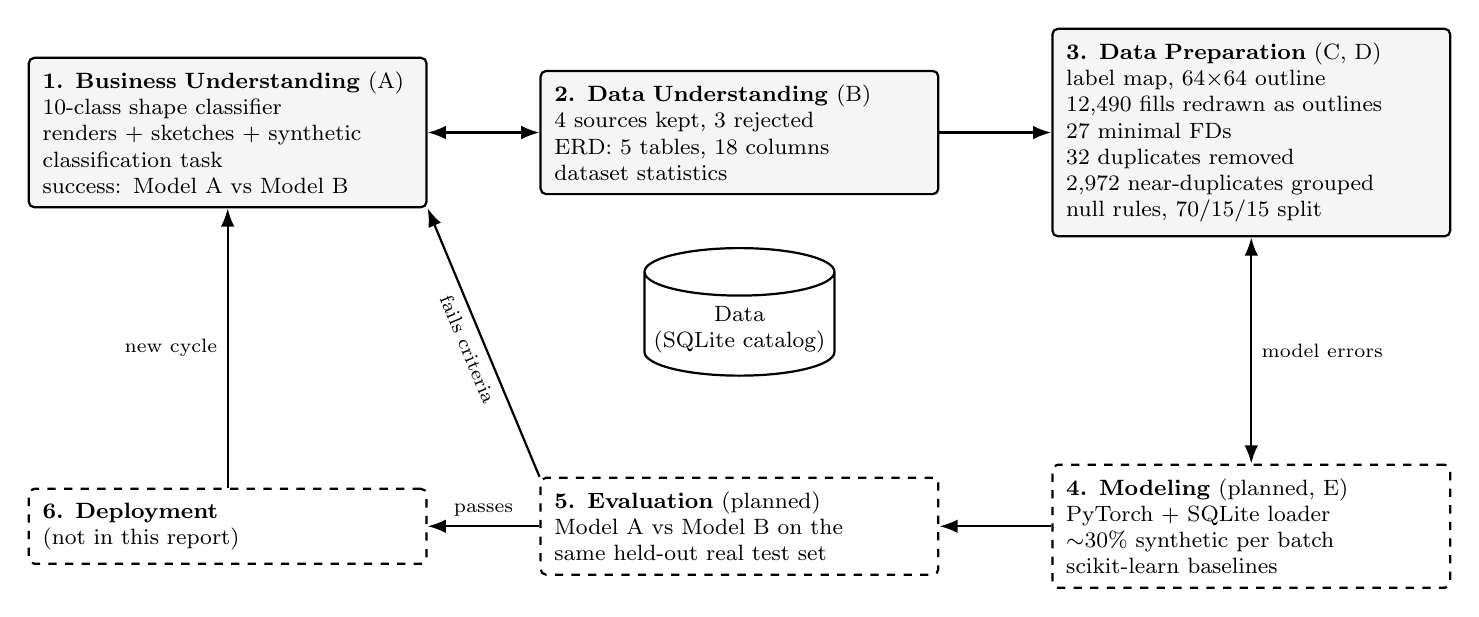
\begin{tikzpicture}[
  box/.style={draw, thick, rounded corners=2pt, fill=gray!8,
              font=\footnotesize, align=left, inner sep=5pt,
              text width=4.7cm},
  plan/.style={box, dashed, fill=white},
  arr/.style={-Latex, thick},
  arr2/.style={Latex-Latex, thick},
  lbl/.style={font=\scriptsize},
]
\node[box]  (bu) at (0,5)     {\textbf{1. Business Understanding} (A)\\
  10-class shape classifier\\ renders + sketches + synthetic\\
  classification task\\ success: Model A vs Model B};
\node[box]  (du) at (6.5,5)   {\textbf{2. Data Understanding} (B)\\
  4 sources kept, 3 rejected\\ ERD: 5 tables, 18 columns\\
  dataset statistics};
\node[box]  (dp) at (13,5)  {\textbf{3. Data Preparation} (C, D)\\
  label map, $64{\times}64$ outline\\ 12,490 fills redrawn as outlines\\
  27 minimal FDs\\ 32 duplicates removed\\
  2,972 near-duplicates grouped\\ null rules, 70/15/15 split};
\node[plan] (mo) at (13,0)  {\textbf{4. Modeling} (planned, E)\\
  PyTorch + SQLite loader\\ $\sim$30\% synthetic per batch\\
  scikit-learn baselines};
\node[plan] (ev) at (6.5,0)   {\textbf{5. Evaluation} (planned)\\
  Model A vs Model B on the\\ same held-out real test set};
\node[plan] (de) at (0,0)     {\textbf{6. Deployment}\\ (not in this report)};
\node[draw, thick, cylinder, shape border rotate=90, aspect=0.25,
      minimum width=2.2cm, minimum height=1.1cm, align=center,
      font=\footnotesize] (data) at (6.5,2.5) {Data\\(SQLite catalog)};

\draw[arr2] (bu) -- (du);
\draw[arr]  (du) -- (dp);
\draw[arr2] (dp) -- node[lbl, right]{model errors} (mo);
\draw[arr]  (mo) -- (ev);
\draw[arr]  (ev) -- node[lbl, above]{passes} (de);
\draw[arr]  (ev.north west) -- node[lbl, below, sloped]{fails criteria} (bu.south east);
\draw[arr]  (de) -- node[lbl, left]{new cycle} (bu);
\end{tikzpicture}}
  \caption{Project mapped onto CRISP-DM \cite[slides 4--5]{lecdp} (solid = done
  for this report, dashed = planned).}
  \label{fig:crisp}
\end{minipage}\hfill
\begin{minipage}[c]{0.32\linewidth}
  \centering
  \resizebox{\linewidth}{!}{%
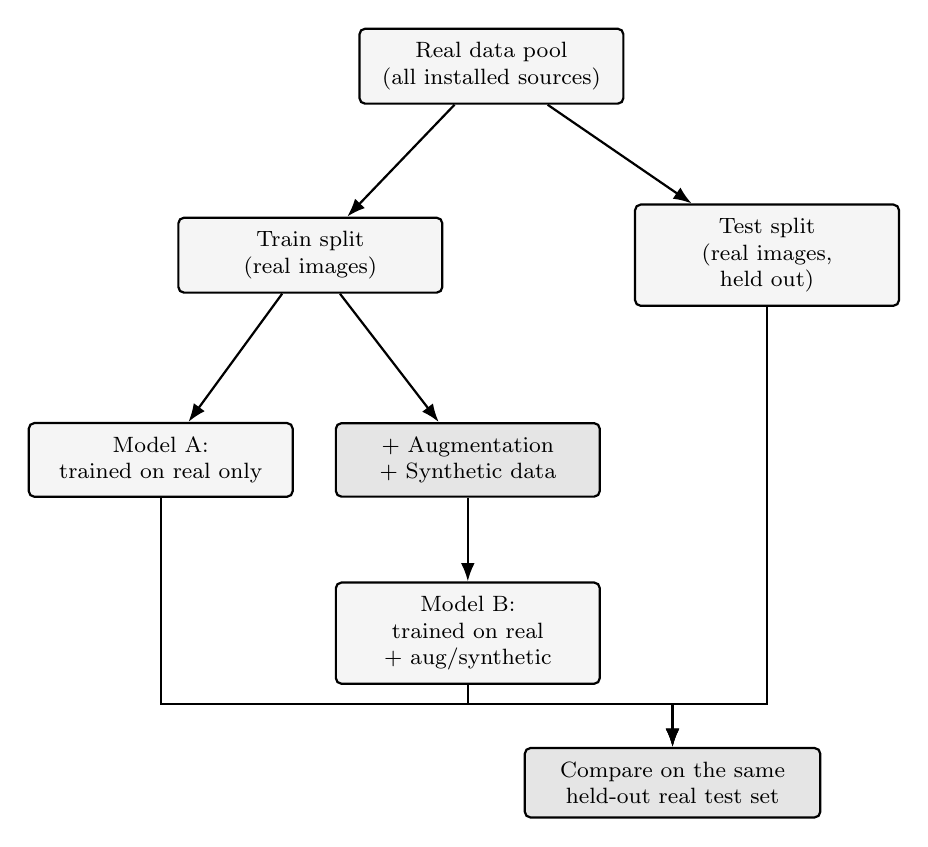
\begin{tikzpicture}[
  box/.style={draw, thick, rounded corners=2pt, fill=gray!8,
              font=\footnotesize, align=center, inner sep=5pt,
              text width=3.0cm},
  arr/.style={-Latex, thick},
]
\node[box]                               (pool)   at (4.5,10)  {Real data pool\\(all installed sources)};
\node[box]                               (train)  at (2.2,7.6) {Train split\\(real images)};
\node[box]                               (test)   at (8.0,7.6) {Test split\\(real images,\\held out)};
\node[box]                               (modelA) at (0.3,5.0) {Model A:\\trained on real only};
\node[box, fill=gray!20]                 (augbox) at (4.2,5.0) {+ Augmentation\\+ Synthetic data};
\node[box]                               (modelB) at (4.2,2.8) {Model B:\\trained on real\\+ aug/synthetic};
\node[box, fill=gray!20, text width=3.4cm] (compare) at (6.8,0.9) {Compare on the same\\held-out real test set};

\draw[arr] (pool) -- (train);
\draw[arr] (pool) -- (test);
\draw[arr] (train) -- (modelA);
\draw[arr] (train) -- (augbox);
\draw[arr] (augbox) -- (modelB);

% Routing to the comparison node
\draw[arr] (modelA.south) -- (0.3,1.9) -- (6.8,1.9) -- (compare.north);
\draw[arr] (modelB.south) -- (4.2,1.9) -- (6.8,1.9) -- (compare.north);
\draw[arr] (test.south)   -- (8.0,1.9) -- (6.8,1.9) -- (compare.north);
\end{tikzpicture}}
  \caption{Evaluation design.}
  \label{fig:evalsplit}
\end{minipage}
\end{figure}


\newpage

% =====================================================================
\section*{B. Summary of the Collected Datasets}
\addcontentsline{toc}{section}{B. Summary of the Collected Datasets}
% =====================================================================

\begin{figure}[H]
\centering
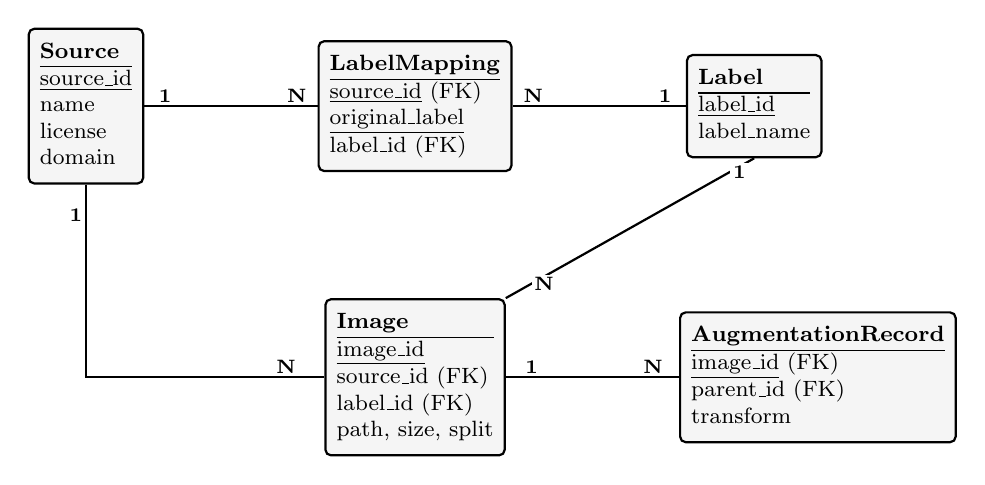
\begin{tikzpicture}[
  ent/.style={draw, thick, rounded corners=2pt, fill=gray!8,
              font=\footnotesize, inner sep=4pt},
  rel/.style={-, thick},
  card/.style={font=\scriptsize\bfseries, fill=white, inner sep=1pt},
]
\node[ent] (src) {\entity{Source}{\underline{source\_id}\\ name\\ license\\ domain}};
\node[ent, right=2.2cm of src] (map) {\entity{LabelMapping}{\underline{source\_id} (FK)\\ \underline{original\_label}\\ label\_id (FK)}};
\node[ent, right=2.2cm of map] (lab) {\entity{Label}{\underline{label\_id}\\ label\_name}};
\node[ent, below=1.6cm of map] (img) {\entity{Image}{\underline{image\_id}\\ source\_id (FK)\\ label\_id (FK)\\ path, size, split}};
\node[ent, right=2.2cm of img] (aug) {\entity{AugmentationRecord}{\underline{image\_id} (FK)\\ parent\_id (FK)\\ transform}};

\draw[rel] (src) -- node[card, pos=0.12, above]{1} node[card, pos=0.88, above]{N} (map);
\draw[rel] (lab) -- node[card, pos=0.12, above]{1} node[card, pos=0.88, above]{N} (map);
\draw[rel] (src.south) |- node[card, pos=0.08, left]{1} node[card, pos=0.92, above]{N} (img.west);
\draw[rel] (lab.south) -- node[card, pos=0.1, right]{1} node[card, pos=0.9, right]{N} (img.north east);
\draw[rel] (img.east) -- node[card, pos=0.15, above]{1} node[card, pos=0.85, above]{N} (aug.west);
\end{tikzpicture}
\caption{ERD of the unified dataset (underlined = key, FK = foreign
key) ,built as a sqlite catalog: 5 tables, 18 columns.}
\label{fig:erd}
\end{figure}

\textbf{Serving.} sqlite holds all the metadata (paths, labels); a custom
loader queries it per batch and applies augmentation and synthetic
generation on the fly. Synthetic images make up about 30\% of each
training batch and we dont store them on disk . 

\textbf{Data sources used.} Four public datasets, verified on disk:
Quick, Draw! \cite{quickdraw} (sketch;  500 drawings for each of the 7
matching categoreis out of 345), reevald's \emph{Geometric Shapes
Mathematics} \cite{kagglereevald} (render), El Korchi's 2D geometric
shapes \cite{elkorchi} (render; only source of pentagons) and the
Hand-Drawn Shapes dataset \cite{handdrawn} (sketch;  only source of
ellipses).

\textbf{Evaluated and not used.} Dinesh \cite{dinesh}: license is
``Unknown'', and its circles, squares and triangles are already
covered anyway. Mendeley \cite{mendeley1,mendeley2}: fully synthetic, none of the
missing classes. swastikarajkower \cite{kaggleswastika}: this turned out to be just a CSV, not
images at all!

\begin{table}[H]
\centering
\caption{Dataset statistics (measured).}
\label{tab:stats}
\small
\begin{tabular}{@{}llrrrrr@{}}
\toprule
Source & Domain & \# files & \# tables & \# columns & Size (MB) & Classes used \\
\midrule
Quick, Draw! (subset) & sketch & 3{,}500 & 7 & 6 & 1.0 & 7 of 7 \\
Kaggle reevald        & render & 20{,}000 & 0 & 0 & 125.1 & 5 of 8 \\
Mendeley El Korchi    & render & 90{,}000 & 0 & 0 & 85.7 & 7 of 9 \\
Hand-drawn (GitHub)   & sketch & 27{,}292 & 20{,}005 & 2 & 47.5 & 3 of 4 \\
\midrule
\textbf{Unified (built)} & mixed & 18{,}500 & 5 & 18 & 12.1 & 10 of 10 \\
\bottomrule
\end{tabular}
\end{table}

\noindent Quick, Draw! has one NDJSON table per category; reevald and El
Korchi dont have any metadata (labels just come from folder or file names); the
hand-drawn set has one vertex table ($x$, $y$) per image. Each
source/class pair is capped at 1,000 images so one source dosent dominate .

\begin{figure}[H]
\centering
\begin{minipage}[c]{0.64\linewidth}
  \centering
  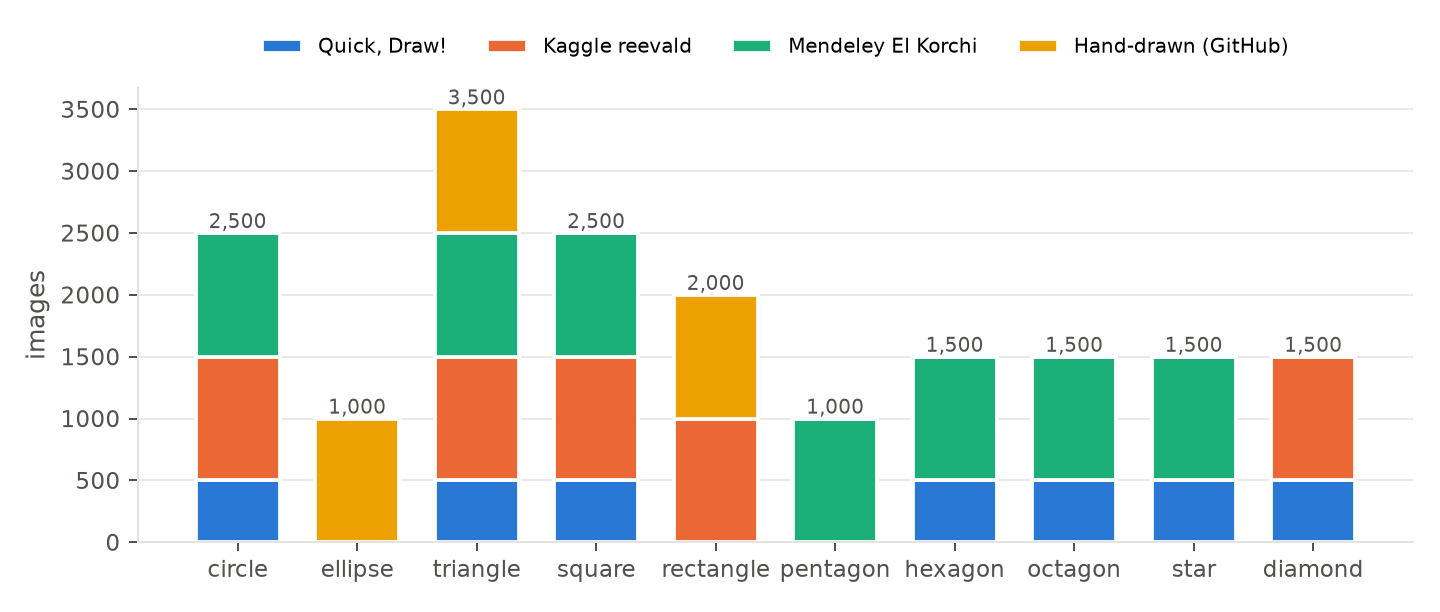
\includegraphics[width=\linewidth]{figures/unified_class_source_counts.png}
  \caption{Images per class, by source.}
  \label{fig:classcounts}
\end{minipage}\hfill
\begin{minipage}[c]{0.32\linewidth}
  \centering
  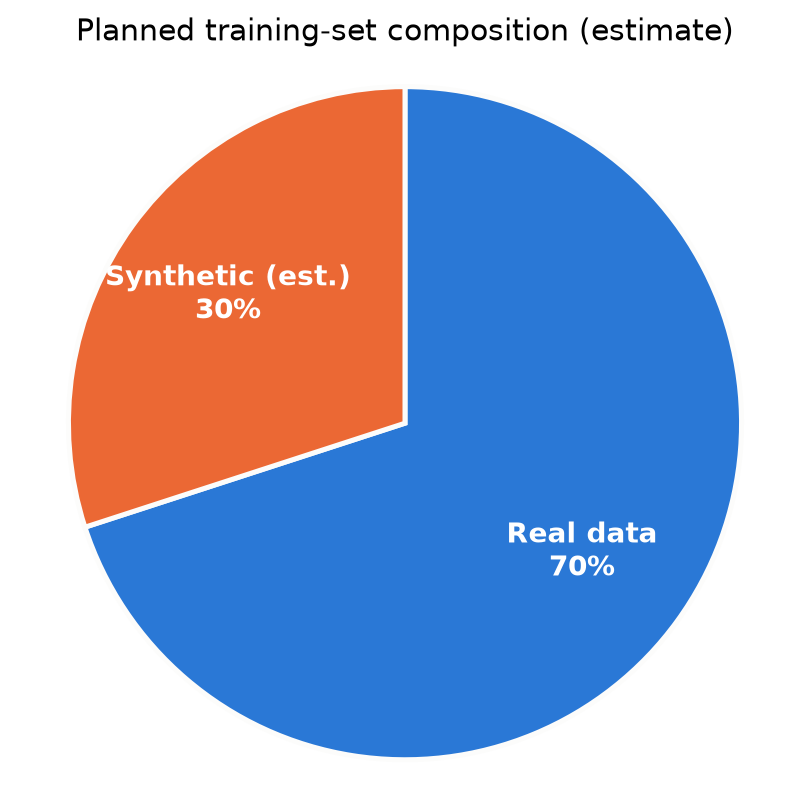
\includegraphics[width=0.85\linewidth]{figures/real_vs_synthetic_pie.png}
  \caption{Planned batch mix: 70\% real, 30\% synthetic.}
  \label{fig:realsynthpie}
\end{minipage}
\end{figure}



% =====================================================================
\section*{C. Data Integration}
\addcontentsline{toc}{section}{C. Data Integration}
% =====================================================================

\textbf{Process.} Every image goes through a single cleaning function
(\nolinkurl{scripts/standardize.py}) and comes out $64{\times}64$,
single channel, black outline on white, centered, with aspect ratio kept . 
Order: map labels $\to$ standardize $\to$ remove duplicates $\to$ split
$\to$ write images, metadata and catalog
(\nolinkurl{scripts/build_unified_dataset.py}).

\begin{table}[H]
\centering
\caption{Integration cases (schema differences in names, coverage and
format \cite[slide 35]{lecfd}).}
\label{tab:cases}
\small
\begin{tabularx}{\linewidth}{@{}p{2.6cm} p{5cm} X@{}}
\toprule
Case & Found in & Resolution \\
\midrule
Dimensions & 256, 224, 200 and 70 px &
  crop, pad to square, resize to $64{\times}64$ \\
Color mode & RGB, RGBA, vector strokes &
  flatten transparency on white; draw strokes 3 px wide \\
Background & random colors (El Korchi); shape lighter or darker &
  shape = pixels far from the background color, adaptive threshold \\
Fill vs outline & fills, dashed outlines, strokes &
  closed shapes redrawn as a 2-px outline; open or dashed strokes kept \\
Scale & shapes down to $\sim$10 px & crop before resizing \\
Label names & \texttt{rhombus}, \texttt{Heptagon}, \texttt{other} &
  label map (Table~\ref{tab:mapping}) \\
Duplicates & identical after standardizing & 32 removed before split \\
\bottomrule
\end{tabularx}
\end{table}

\textbf{Filled shapes need a conversion filter.} El Korchi and Dinesh
have filled shapes on colored backgrounds, while sketches are just outlines.
If we left them as is, the fill would give away the source instead of the actual shape, so our
filter redraws them as outlines (Figure~\ref{fig:filloutline}). In total, 12,490
images (67.5\%) were redrawn . One small limitation: reevald's dashed lines still sort of hint at
where they came from.

\begin{figure}[H]
\centering
\begin{minipage}[b]{0.3\linewidth}
  \centering
  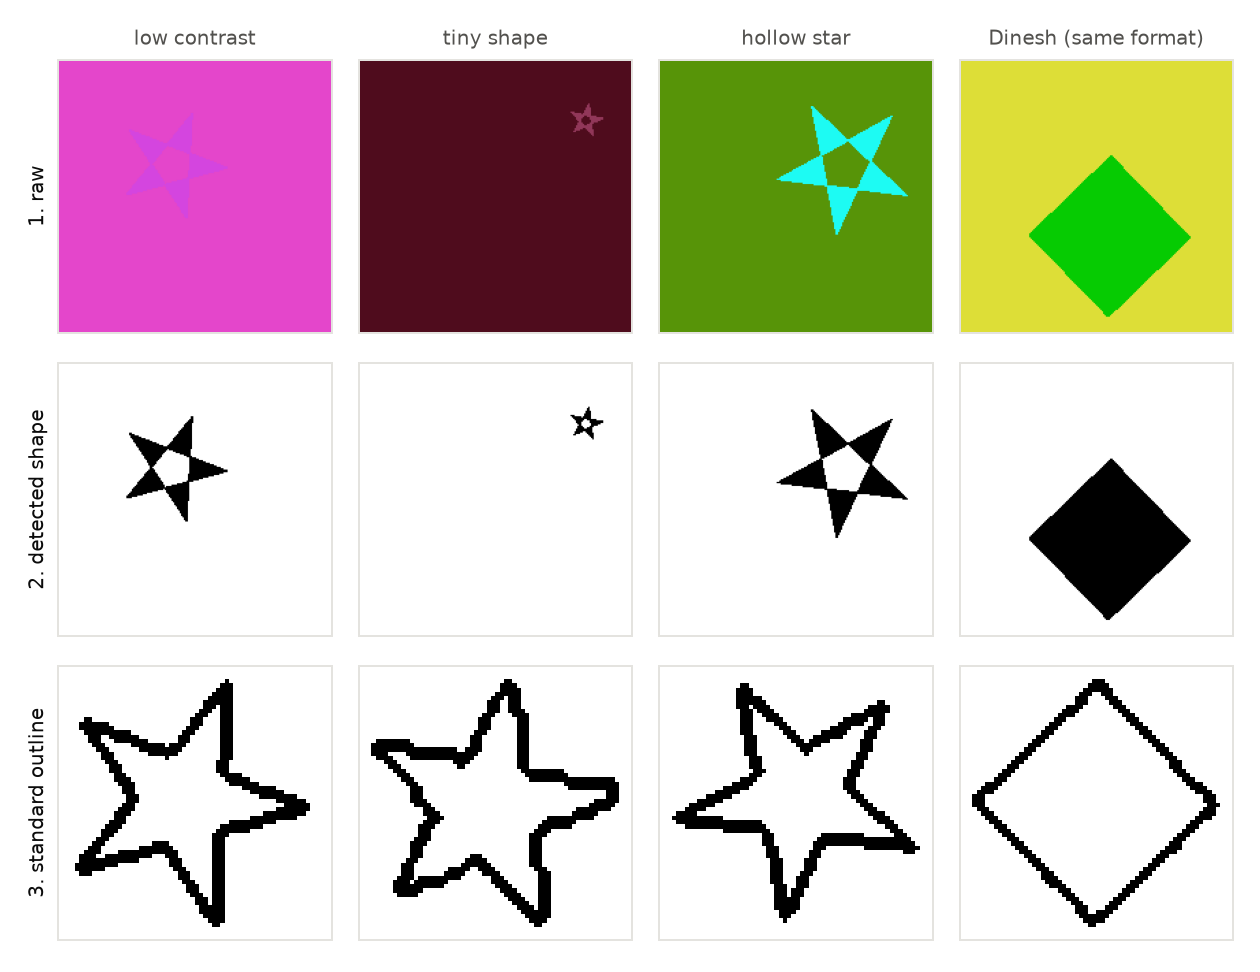
\includegraphics[width=\linewidth]{figures/fill_to_outline.png}
  \caption{Conversion filter on hard cases: raw, detected shape,
  outline.}
  \label{fig:filloutline}
\end{minipage}\hfill
\begin{minipage}[b]{0.6\linewidth}
  \centering
  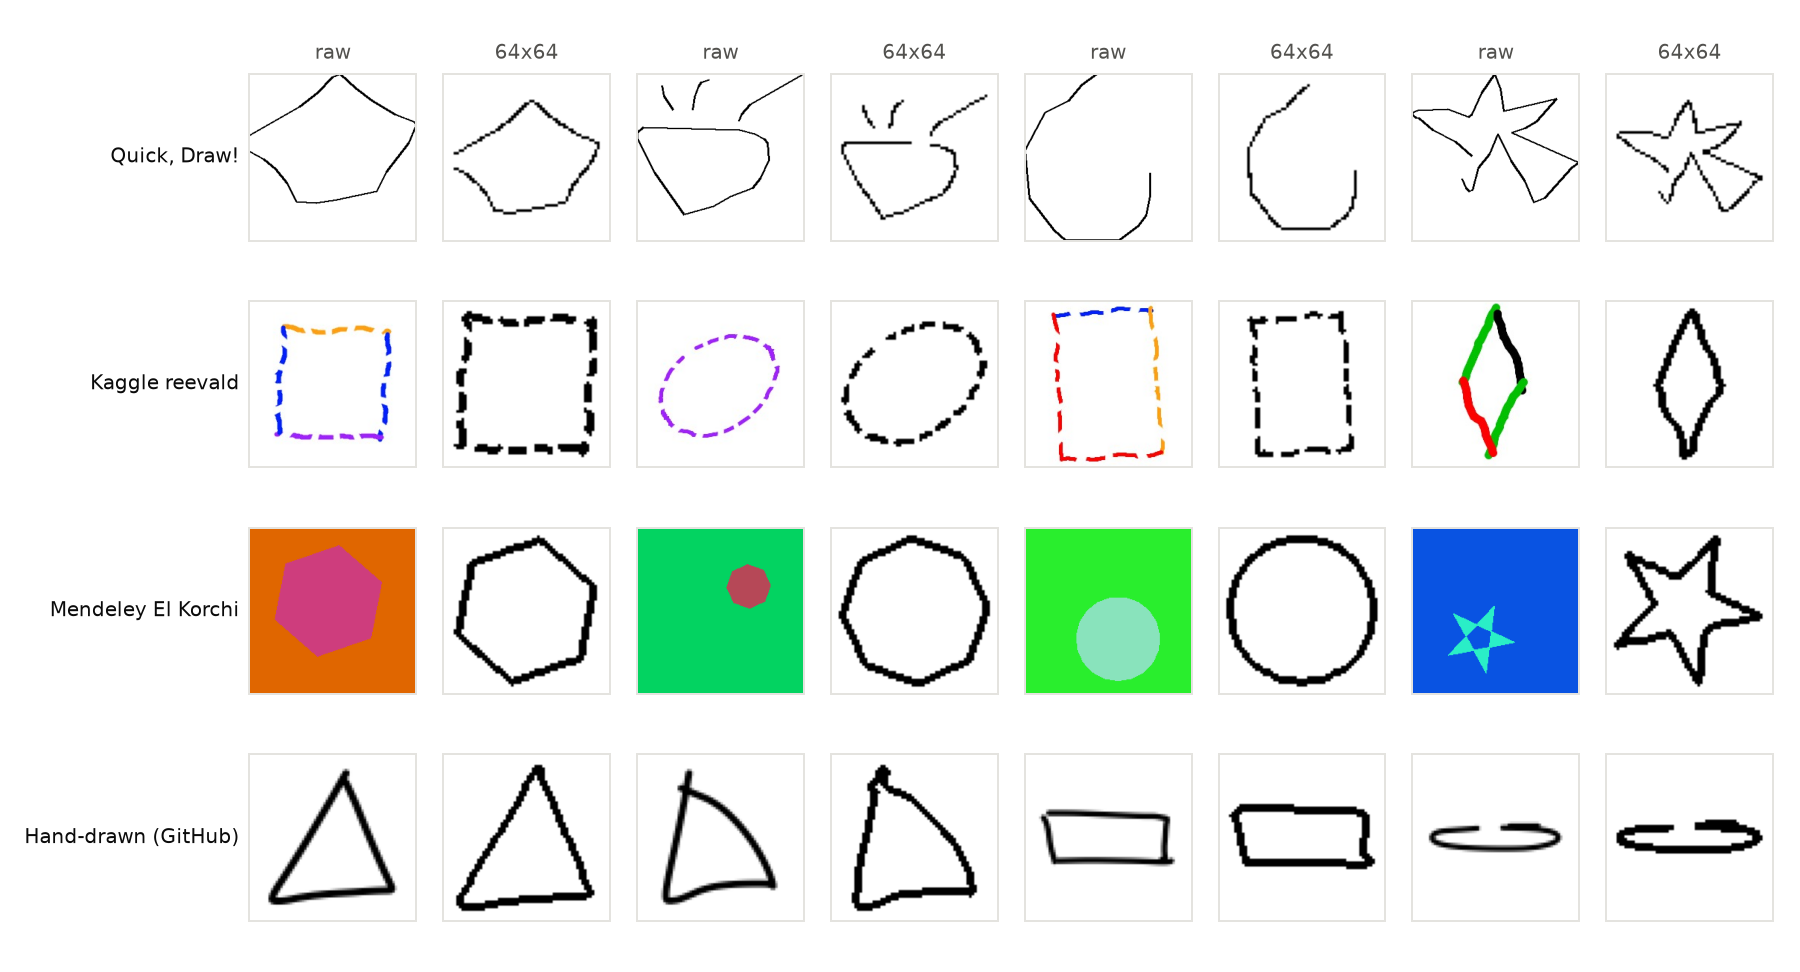
\includegraphics[width=\linewidth]{figures/standardization_before_after.png}
  \caption{Raw vs standardized, per source.}
  \label{fig:beforeafter}
\end{minipage}
\end{figure}

\begin{table}[H]
\centering
\caption{Label mapping.}
\label{tab:mapping}
\small
\begin{tabular}{@{}llll@{}}
\toprule
Source & Original label & Unified label & Action \\
\midrule
Kaggle reevald  & \texttt{rhombus}       & diamond & merge synonym \\
Kaggle reevald  & \texttt{kite}, \texttt{trapezoid}, \texttt{parallelogram} & -- & drop (out of taxonomy) \\
El Korchi       & \texttt{Pentagon}, \texttt{Star}, \dots & pentagon, star, \dots & normalize case \\
El Korchi       & \texttt{Heptagon}, \texttt{Nonagon} & -- & drop (out of taxonomy) \\
Hand-drawn      & \texttt{other}         & --      & drop (not a shape class) \\
Quick, Draw!    & \texttt{diamond}       & diamond & keep (includes gemstones, see D) \\
\bottomrule
\end{tabular}
\end{table}

\textbf{Functional dependencies.} A script tested every 1- and
2-column left-hand side over 11 metadata columns of the 18,500 unified
rows and found 27 minimal FDs (\nolinkurl{scripts/discover_fds.py}).
Table~\ref{tab:fdcheck} shows the meaningful ones; three were not
designed. No approximate FDs (under 5\% error) were found. An injected
wrong \texttt{label\_id} was caught (\nolinkurl{scripts/check_fds.py}),
using FDs to detect inconsistencies \cite[slide 20]{lecfd}.

\begin{table}[H]
\centering
\caption{Discovered functional dependencies (18,500 rows).}
\label{tab:fdcheck}
\small
\begin{tabularx}{\linewidth}{@{}>{\raggedright\arraybackslash}p{5.2cm} l
  >{\raggedright\arraybackslash}X@{}}
\toprule
Dependency & Origin & What it shows \\
\midrule
\fd{source\_id}{(domain, license)} & by design & -- \\
\fd{label\_id}{label\_name} (and back) & by design & -- \\
\fd{original\_label}{label\_id} & discovered & no label name maps to
  two classes across sources; the designed key (source, label) is
  larger than needed \\
\fd{native\_width}{source\_id} & discovered & image size alone reveals
  the source, a shortcut the resize to $64{\times}64$ removes \\
\fd{(source\_id, label\_id)}{original\_label} & discovered & each
  source uses one name per class \\
\bottomrule
\end{tabularx}
\end{table}



% =====================================================================
\section*{D. Data Preparation}
\addcontentsline{toc}{section}{D. Data Preparation}
% =====================================================================

\textbf{Null data.} Mapped onto our schema, every source is missing some
fields. Our rules: no label $\to$ drop; no size $\to$ derive it; no
license $\to$ \texttt{unknown} (source excluded). Dropping rows without
a class label and filling a global constant follow \cite[slide 24]{lecdp}.

\begin{table}[H]
\centering
\caption{Real null cases when mapping sources onto the schema.}
\small
\begin{tabularx}{\linewidth}{@{}>{\raggedright\arraybackslash}p{4.4cm}
  >{\raggedright\arraybackslash}p{4.4cm}
  >{\raggedright\arraybackslash}X r@{}}
\toprule
Source & Missing field & Handling & Images \\
\midrule
reevald, El Korchi, hand-drawn & \texttt{label\_id} (no matching
  class) & dropped: kite, trapezoid, parallelogram, heptagon, nonagon,
  other & 34{,}787 \\
reevald, El Korchi, hand-drawn & label (no metadata) & taken from folder or
  file name & all \\
Quick, Draw! & width, height (vector strokes) & drawn on a
  $256{\times}256$ canvas & 3{,}500 \\
all sources & per-image license & inherited from the \emph{Source} table &
  all \\
Dinesh & license (``Unknown'') & \texttt{unknown}, source excluded &
  30{,}000 \\
\bottomrule
\end{tabularx}
\end{table}

\textbf{Outlier detection.} Results from our build:
\begin{itemize}
  \item \textbf{No contrast:} 1 image got rejected, the shape was the exact same color as
        its background (Figure~\ref{fig:outliers}, top).
  \item \textbf{Exact duplicates:} 32 identical images were removed before the split.
  \item \textbf{Near duplicates:} 2,972 images ended up in near-identical groups
        (perceptual hash \cite{zauner}); each group stays in one split so data dosent leak.
  \item \textbf{Low diversity:} El Korchi shapes mostly differ in color,
        size and position, which standardisation removes; one group alone holds
        175 near-identical pentagons (Figure~\ref{fig:outliers}, bottom).
  \item \textbf{Not yet filtered:} Quick, Draw!'s \texttt{diamond}
        still includes some gemstone drawings that we might filter later..
\end{itemize}

\begin{figure}[H]
\centering
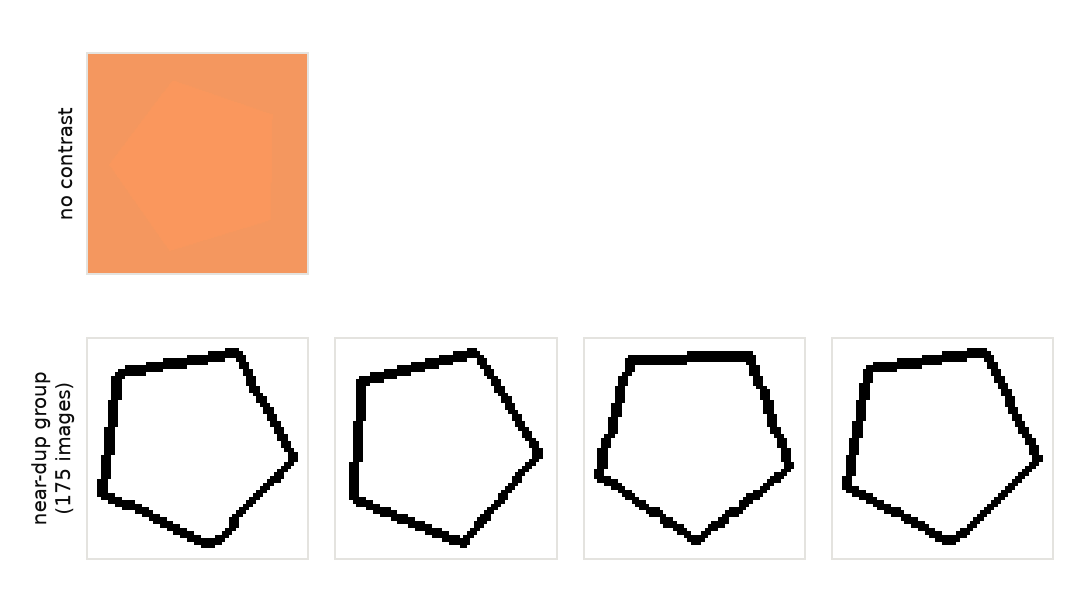
\includegraphics[width=0.55\linewidth]{figures/outlier_examples.png}
\caption{Top: rejected (no contrast). Bottom: a near-duplicate group of
175 pentagons.}
\label{fig:outliers}
\end{figure}

\textbf{Split.} 70/15/15 split by near-duplicate group: 12,761 train, 2,890
validation, 2,849 test. Augmentation and synthetic data strictly come after the
split, on the training set only \cite{lones}\cite[slide 58]{lecclf}.

\textbf{Transformation.} Images are stored as $64{\times}64$ 8-bit PNGs,
normalized to $[0,1]$ on load; labels use their index
(table~\ref{tab:labels}). Training images (real and synthetic) get five
augmentations \cite{labellerr}: rotation, scale, shear, noise, blur . 
Shear and non-uniform scaling are disabled for circle, ellipse, square,
rectangle and diamond, since those transforms would actually chnage the geometric class!

\begin{figure}[H]
\centering
\begin{minipage}[b]{0.48\linewidth}
  \centering
  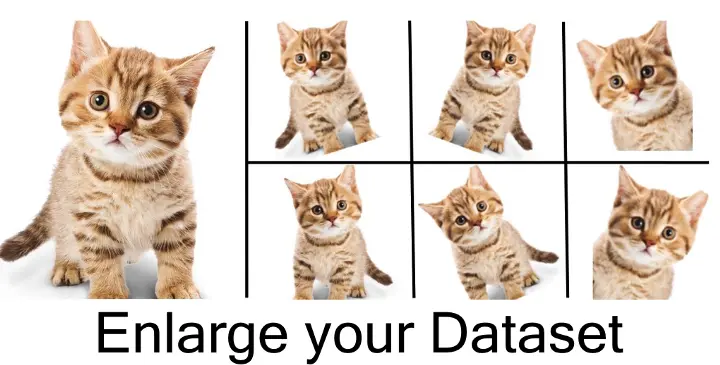
\includegraphics[width=\linewidth]{figures/data_augmentation_example.png}
  \caption{Augmentation examples (adapted from \cite{labellerr}).}
  \label{fig:augexample}
\end{minipage}\hfill
\begin{minipage}[b]{0.48\linewidth}
  \centering
  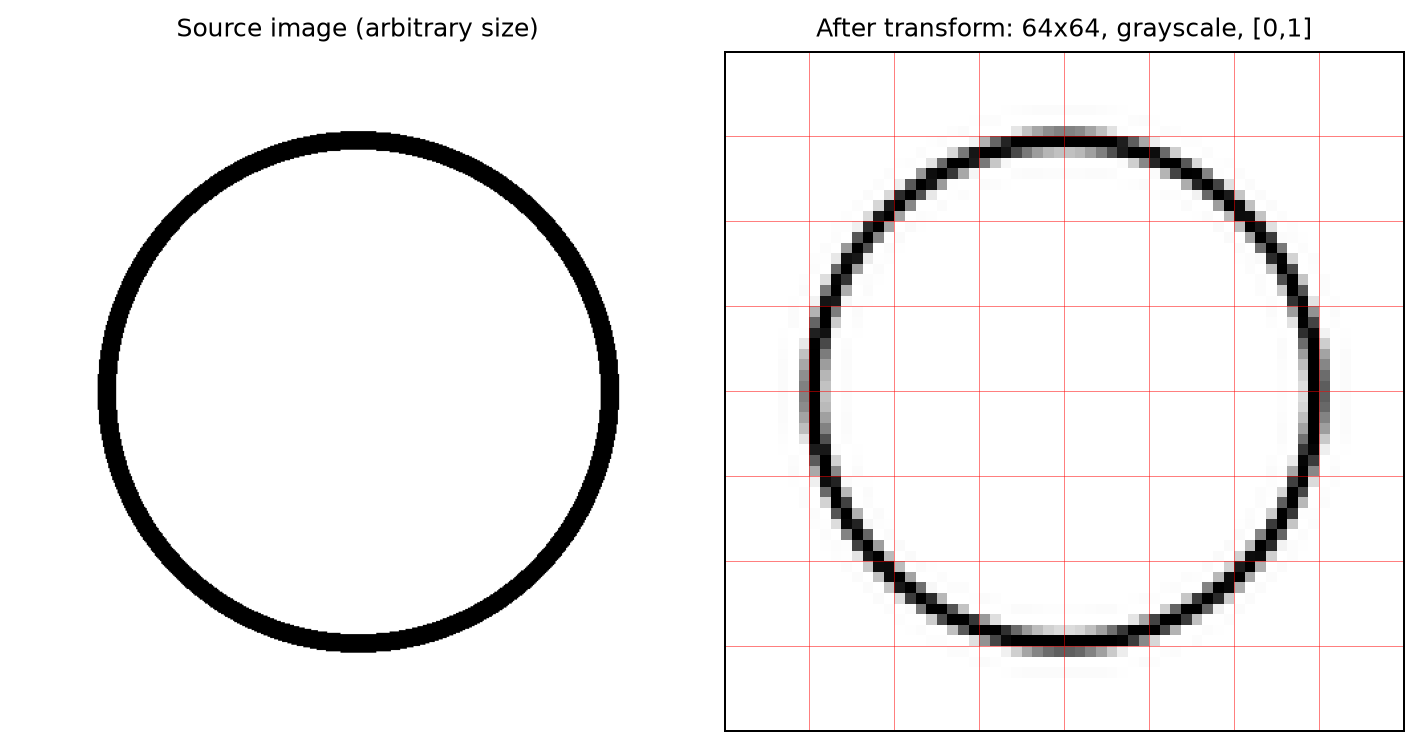
\includegraphics[width=\linewidth]{figures/transform_pixel_grid.png}
  \caption{A circle before and after resizing to the $64\times64$
  grid.}
  \label{fig:pixelgrid}
\end{minipage}
\end{figure}



% =====================================================================
\section*{E. Tools and Systems}
\addcontentsline{toc}{section}{E. Tools and Systems}
% =====================================================================

\begin{table}[H]
\centering
\caption{Tools by role: in use (already built the dataset) or planned (training) .}
\small
\begin{tabularx}{\linewidth}{@{}X X l@{}}
\toprule
Role & Tool & Status \\
\midrule
Image I/O, rasterization & Pillow & in use \\
Masking, morphology, perceptual hash & NumPy, SciPy & in use \\
Database serving & SQLite & in use \\
Metadata and FD checks & Python scripts (\texttt{scripts/}) & in use \\
Visualization and QA & Matplotlib & in use \\
Version control & Git & in use \\
Synthetic rendering & Pillow ImageDraw & planned \\
Augmentation & Albumentations & planned \\
Training & PyTorch with a custom on-demand data loader & planned \\
Baselines & scikit-learn & planned \\
\bottomrule
\end{tabularx}
\end{table}



\newpage
% =====================================================================
\begin{thebibliography}{9}
\bibitem{quickdraw} Google Creative Lab. \emph{The Quick, Draw! Dataset}.
  License: CC BY 4.0.
  \url{https://github.com/googlecreativelab/quickdraw-dataset}
\bibitem{kagglereevald} reevald. \emph{Geometric Shapes Mathematics}.
  Kaggle. License: CC0, public domain.
  \url{https://www.kaggle.com/datasets/reevald/geometric-shapes-mathematics}
\bibitem{elkorchi} A. El Korchi. \emph{2D geometric shapes dataset}.
  Mendeley Data, DOI 10.17632/wzr2yv7r53.1. License: CC BY 4.0.
  \url{https://data.mendeley.com/datasets/wzr2yv7r53/1}
\bibitem{handdrawn} frobertpixto. \emph{Hand-Drawn Shapes Dataset}.
  GitHub. License: CC BY 4.0 (data), MIT (code).
  \url{https://github.com/frobertpixto/hand-drawn-shapes-dataset}
\bibitem{dinesh} dineshpiyasamara. \emph{Geometric Shapes Dataset}.
  Kaggle. License: stated as ``Unknown'' (excluded).
  \url{https://www.kaggle.com/datasets/dineshpiyasamara/geometric-shapes-dataset}
\bibitem{mendeley1} Mendeley Data. \emph{2D Geometric shapes with
  properties} (synthetic, 7 base shapes; not used). License: CC BY 4.0.
  \url{https://data.mendeley.com/datasets/d35tjjgjnx/1}
\bibitem{mendeley2} S. Dolgikh. \emph{Geometrical shapes datasets}
  (synthetic, circles/triangles; not used). Mendeley Data. License:
  CC BY 4.0.
  \url{https://data.mendeley.com/datasets/ypfcrfxjgk/1}
\bibitem{kaggleswastika} swastikarajkower. \emph{Geometric Shapes
  Classification Dataset} (CSV of shape measurements, not images; not
  used). Kaggle. No license stated.
  \url{https://www.kaggle.com/datasets/swastikarajkower/geometric-shapes-classification-dataset}
\bibitem{zauner} C. Zauner. \emph{Implementation and Benchmarking of
  Perceptual Image Hash Functions}. Master's thesis, 2010.
  \url{https://phash.org/docs/pubs/thesis_zauner.pdf}
\bibitem{lones} M. A. Lones. \emph{How to avoid machine learning
  pitfalls: a guide for academic researchers}. arXiv:2108.02497.
  \url{https://arxiv.org/abs/2108.02497}
\bibitem{labellerr} Labellerr. \emph{Data Augmentation: Train Deep
  Learning Models with Limited Data}.
  \url{https://www.labellerr.com/blog/data-augmentation-train-deep-learning-models-with-limited-data/}
\bibitem{lecdp} E. Mansour. COMP 333 lecture \emph{Introduction to Data
  Analysis: Data Preparation} (W4\_DP\_P1.pdf).
\bibitem{lecfd} E. Mansour. COMP 333 lecture \emph{Introduction to Data
  Analysis: FDs + DI} (W3\_FDs\_DI\_Lec1.pdf).
\bibitem{lecclf} E. Mansour. COMP 333 lecture \emph{Introduction to Data
  Analysis: Machine learning, classification}
  (week-6-lecture-3-classification.pdf).
\end{thebibliography}

\end{document}
